\documentclass[conference]{IEEEtran}
\IEEEoverridecommandlockouts
% The preceding line is only needed to identify funding in the first footnote. If that is unneeded, please comment it out.
\usepackage{cite}
\usepackage{amsmath,amssymb,amsfonts}
\usepackage{algorithmic}
\usepackage{graphicx}
\usepackage{textcomp}
\usepackage{xcolor}
\usepackage{float}
\usepackage{url}
\def\BibTeX{{\rm B\kern-.05em{\sc i\kern-.025em b}\kern-.08em
    T\kern-.1667em\lower.7ex\hbox{E}\kern-.125emX}}
\begin{document}

\title{HOMEWOEK 2}

\author{\IEEEauthorblockN{Runlin Hou}
\IEEEauthorblockA{\textit{ECE, School Of Graduate Studies} \\
\textit{Rutgers University}\\
hourunlinxa@gmail.com}
}

\maketitle

\section*{Trend Line \& Channel}
Trend line, as what it is been called, describes a trend of the price movement of a 
security. It is based on the historical record of the stock you are looking into.

To draw a trend line, the first thing we need to get is the historical data of this
stock. After we plot the data we get, we usually obtain a line chart. Since the price 
will go down and fo up all the time, so we will have local min points and local max 
points, which is been called support point and resistance point. If we fit a line with
three more support points, we get a \textbf{support trend line}. Otherwise, if we fit a line with
three more resistance points, we get a \textbf{resistance trend line}. Between a support line and
a resistance line is a channel, who predicts the whole price trend for us.

\begin{figure}[H]
    \centerline{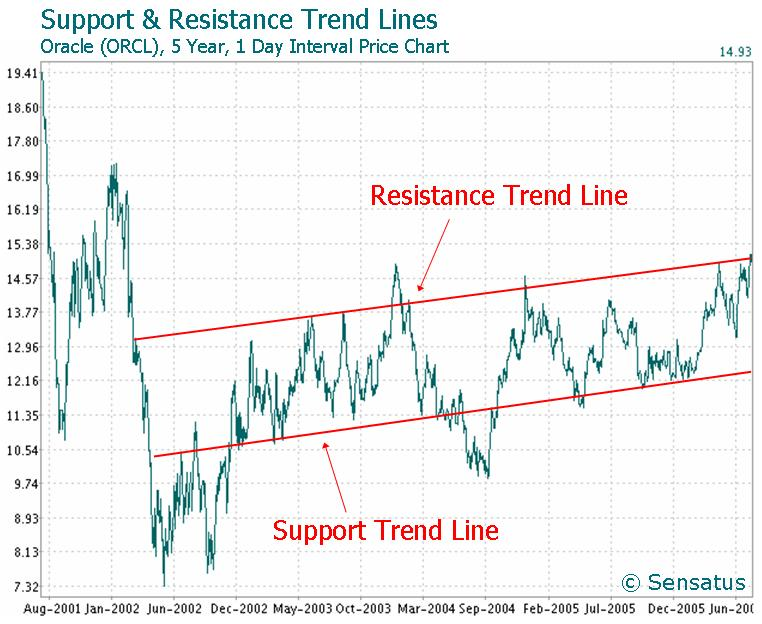
\includegraphics[scale=0.45]{Pic/pic1.jpg}}
    \caption{In this plot the two red lines draw a channel}
\end{figure}

\section*{Major Trend Reversals}
Generally speaking, a major trend reversal means there are two trend exists in a same
chart. It is usually not to be observed at the begining and it is only can be confirmed
after the trend has gone far enough.

\begin{figure}[H]
    \centerline{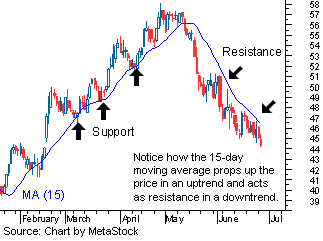
\includegraphics[scale=0.7]{Pic/pic2.png}}
    \caption{A major trend recersal will usually look like this.}
\end{figure}

\section*{Patterns}

\subsection*{Head-and-shoulders Pattern}
This pattern shows a major trend reversal.

Head and Shoulders formation consists of a left shoulder, 
a head, and a right shoulder and a line drawn as the neckline.
Also there is an upside down version of this pattern.

\begin{figure}[H]
    \centerline{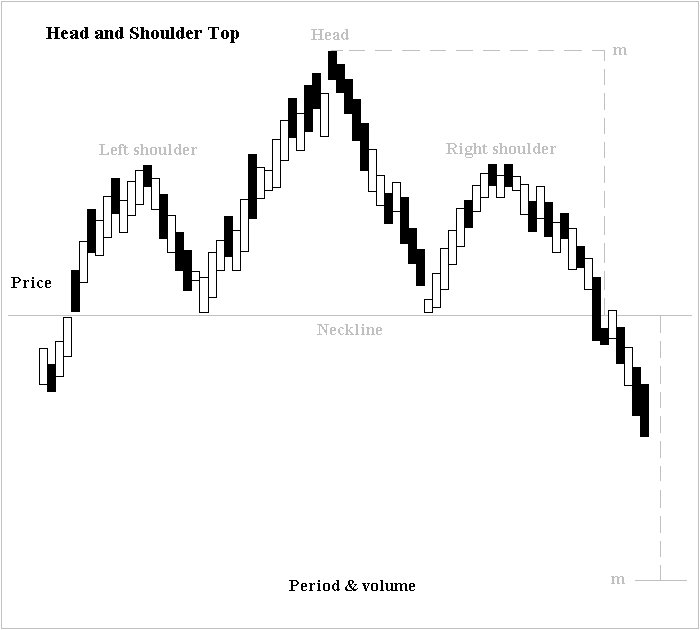
\includegraphics[scale=0.45]{Pic/pic3.jpg}}
    \caption{In this plot the two red lines draw a channel}
\end{figure}


\subsection*{Flags and Pennant Pattern}
The following patterns are different from the Major Trend Reversal. The trend are usually 
tend to be steady and short lasting.

The flag pattern is encompassed by two parallel lines. These lines can be either flat or
pointed in the opposite direction of the primary market trend. 

A classic pattern for technical analysts, the pennant pattern is identifiable by a large 
price move, followed by a continuation period and a breakout.

\begin{figure}[H]
    \centerline{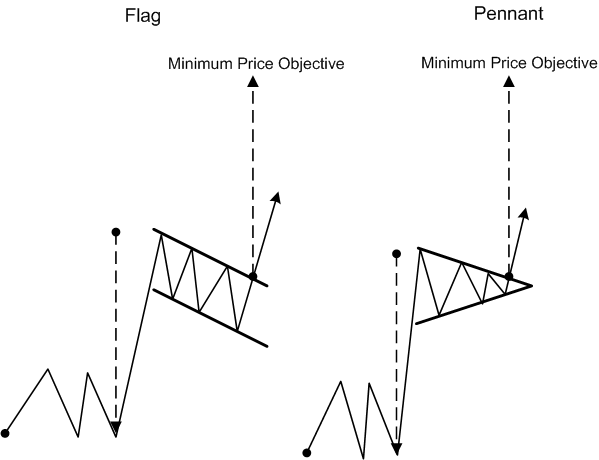
\includegraphics[scale=0.45]{Pic/pic4.png}}
    \caption{This plot shows two different patterns.}
\end{figure}

As we can see in the above graph, there two different patterns are pretty similar to each
other. The difference is that the support trend line and the resistance trend line of flags
pattern are parallel to each other, but the two line of pennant pattern are intersected.

\subsection*{Triangles Pattern}
The pattern derives is name from the fact that it is characterized by a contraction in 
price range and converging trend lines, thus giving it a triangular shape. And the 
triangles are different from each other depends on wether it is ascending or decreasing or neither.

\begin{figure}[H]
    \centerline{\includegraphics[scale=0.05]{Pic/pic5.png}}
\end{figure}

\begin{figure}[H]
    \centerline{\includegraphics[scale=0.05]{Pic/pic6.png}}
\end{figure}

\begin{figure}[H]
    \centerline{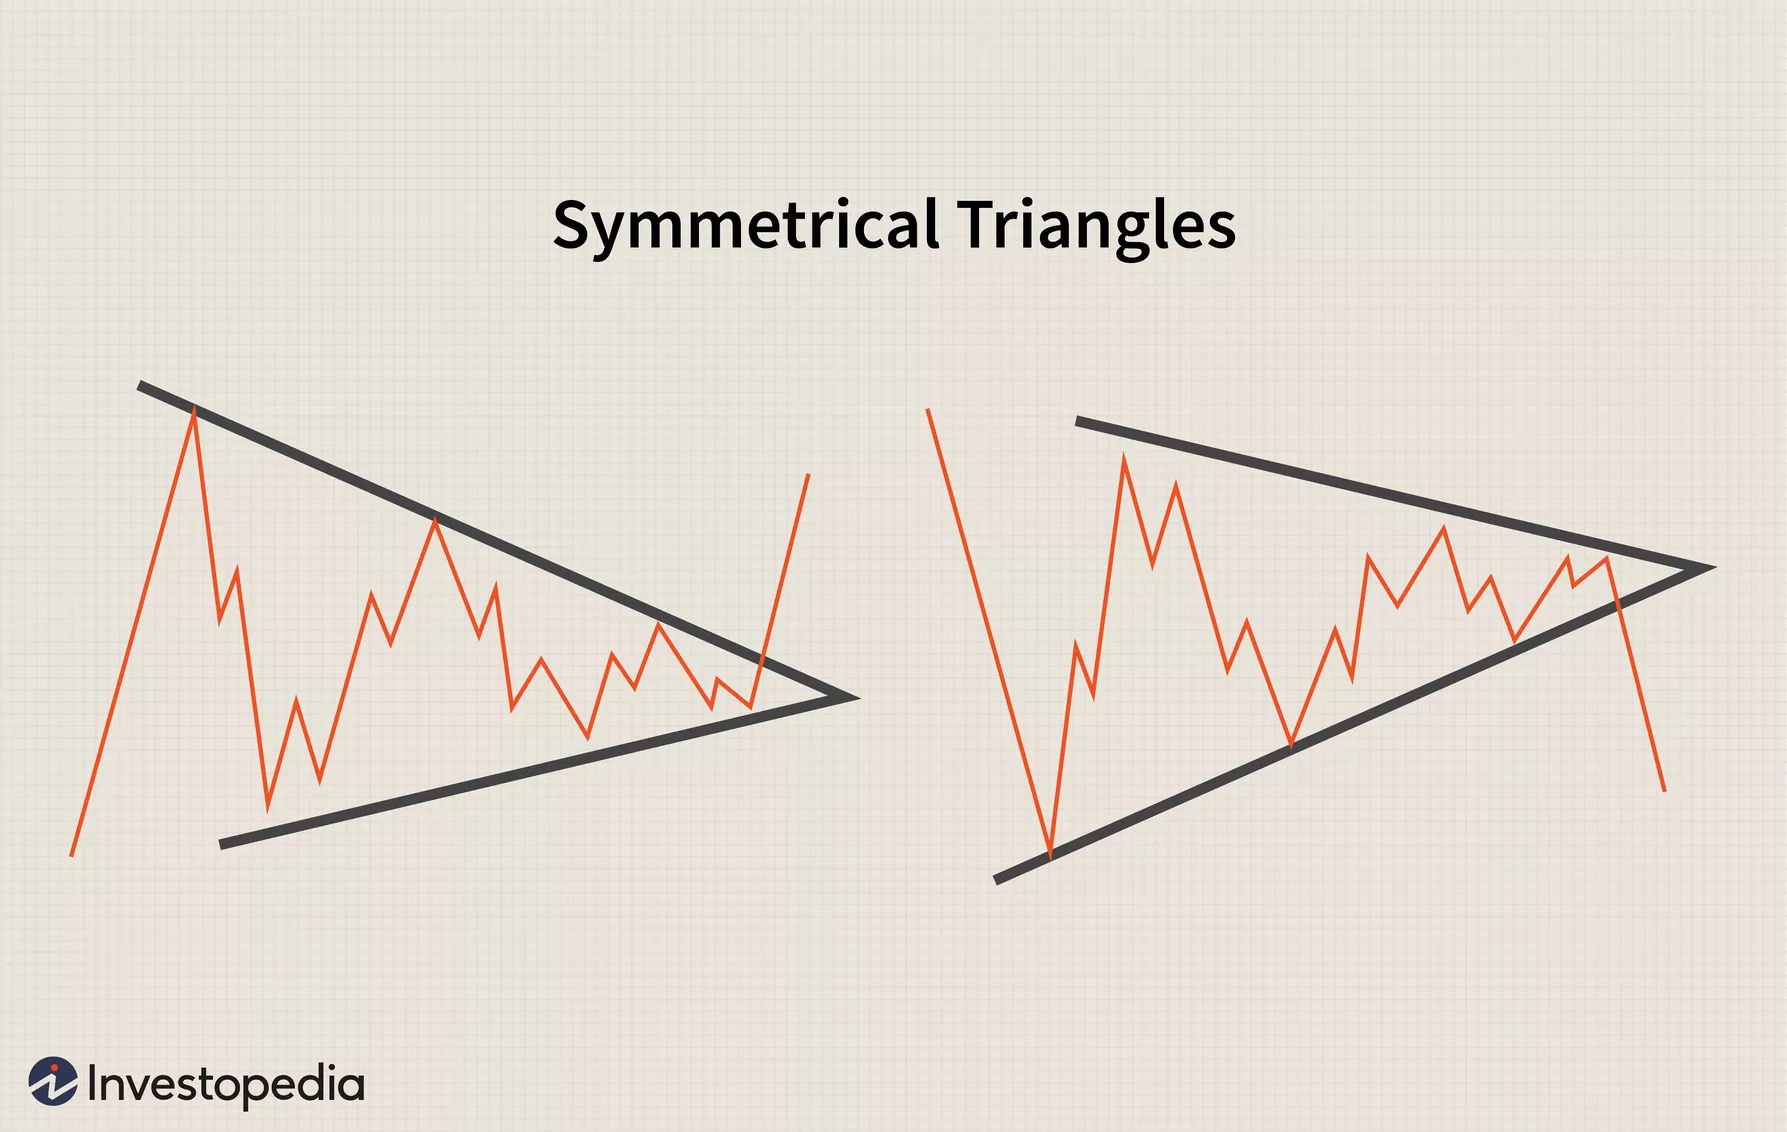
\includegraphics[scale=0.15]{Pic/pic7.png}}
\end{figure}


\begin{thebibliography}{00}
\bibitem{b1} \url{https://en.wikipedia.org/wiki/Trend_line_(technical_analysis)}
\bibitem{b2} \url{https://onlinelibrary.wiley.com/doi/10.1002/9781119202622.ch3}
\bibitem{b3} \url{https://en.wikipedia.org/wiki/Flag_and_pennant_patterns#Flag_pattern}
\bibitem{b4} \url{https://www.investopedia.com/articles/technical/03/091003.asp}
\end{thebibliography}

\end{document}
